%! TeX root = master.tex
% !TEX program = lualatex

\lecture{3}{03-03-26}{Linear Models for Classification (Binary classification)}{}

\begin{definition}[Loss function]
  The loss function (general ML concept) : $l(\hat{y_i}, yi)$ computes an error value between the prediction and the true value.
\end{definition}

\subsection{Logistic regression}

The idea of the logistic regression is that first we compute $y = w^Tx$ and then we apply the sigmoid on y written $\sigma(y)$, to establish a probability $p(y=1|x)$. Then the decision boundary is obtained when the probability equals \left(0.5\right).
\\
\textbf{Logistic function}: $f(a) = \frac{1}{1 + exp(-a)}$ 
\\
Applying it to the output of a linear model gives a prediction:
\[
  \hat{y} = \frac{1}{1 + exp(-w^{(0)} - w^{(1)}x)}
\]
This is a smooth approximation of the step function (avoid the gradient that is zero almost everywhere). 

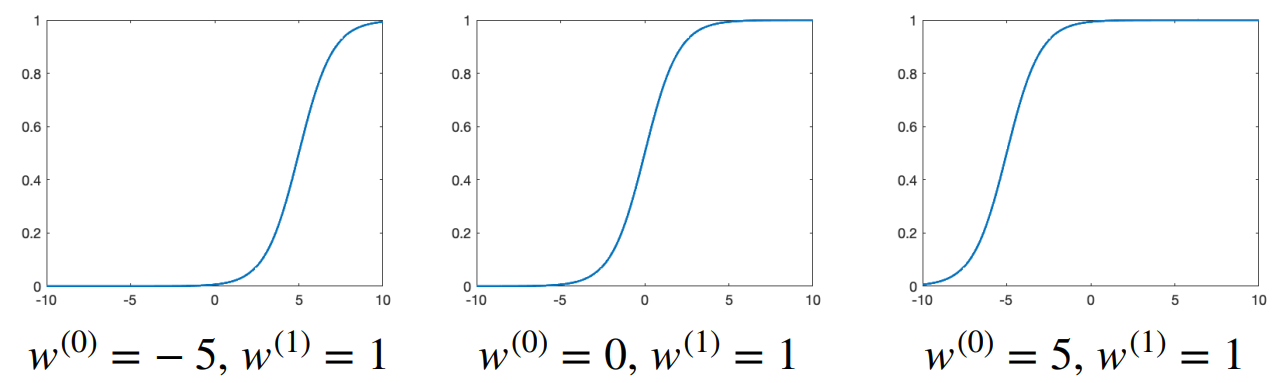
\includegraphics[width=0.5\linewidth]{images/img_20260304_192017.png}
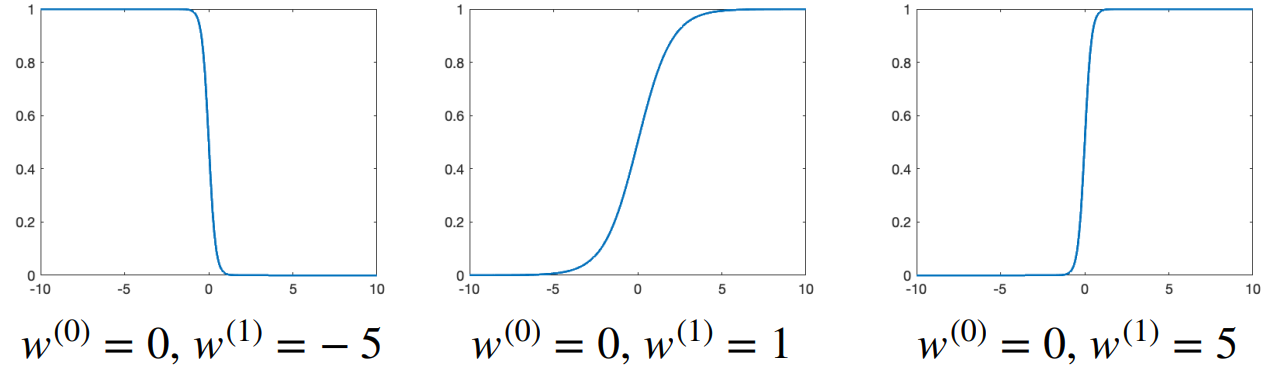
\includegraphics[width=0.5\linewidth]{images/img_20260304_192158.png}
\\

\begin{wrapfigure}{r}{0.4\linewidth}
  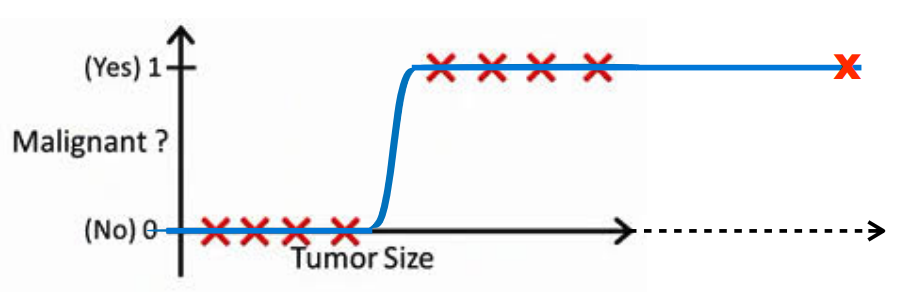
\includegraphics[width=\linewidth]{images/img_20260304_192441.png}\\
\end{wrapfigure}

Then the data fit much better even with the presence of outliers

In the binary case, with $D$ dimensional inputs, we can write the prediction of the model (logistic regression) as
\[
  \hat{y} = \sigma(w^Tx) = \frac{1}{1 + exp(-w^Tx)}
\]
it can be interpreted as the probability that \textbf{x} belongs to the positive class \to  $1 - \hat{y}$ = proba. negative class.
\\ Notes, in the logistic regression: 
\[
  y \in \left\{0, 1\right\} \text{ with } 0 \to \text{negative class, } 1 \to \text{positive class}
\]
\[
  \text{The model computes: } \hat{y} = P\left(y = 1 | x \right)
\]

\\ Even that the name of this model is logistic \textbf{regression}, this is truly a classification model, not a regression one.

\subsubsection{Training}
To learn the parameters \textbf{w} need a loss function: \\
\textbf{Cross-entropy} :

\textbf{1D case}

\[
  R(w) = - \sum_{i = 1}^N  (y_iln(\hat{y_i}) + (1-y_i)ln(1 - \hat{y_i}))
= - \sum_{i \in positive samples} ln(\hat{y_i}) - \sum_{i \in negative samples} ln(1 - \hat{y_i})
\] \to as $y_i$ is either 0 or 1 \\
It's a \textbf{convex} function, however, its minimization has no closed-form solution. So we optimize it via gradient descent.\\
The \textbf{algorithm} for minimization is:
\begin{itemize}
  \item 1. Initialize $w_0$ (e.g, randomly)
  \item 2. While not converged \implies  update $ w_k \leftarrow w_{k-1} - \eta \frac{dR(w_{k-1})}{dw}$ \quad with $\eta$ the step size of each iteration (learning rate)
\end{itemize}

\begin{wrapfigure}{r}{0.3\linewidth}
  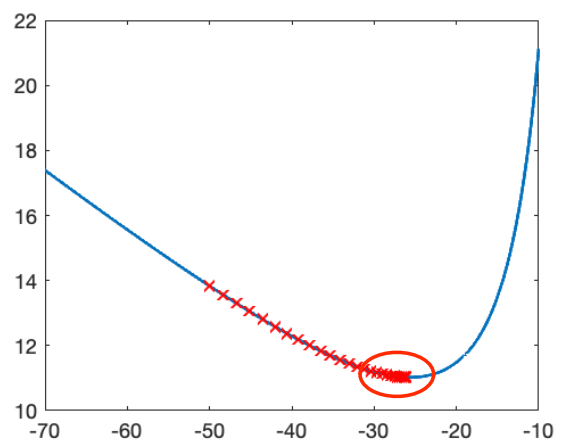
\includegraphics[width=\linewidth]{images/img_20260304_195123.png}
\end{wrapfigure}

This algorithm converges because the derivative becomes smaller $(\frac{dR(w)}{dw} \to  0$ ($\nabla w$ becomes smaller)).\\
The $\eta$ influences the speed of the convergences (doing bigger or smaller steps), but having too large steps may make the algorithm to jumps between two points and never converge. \\
As the initial $w_0$ is the starting point, having a $w_0$ near the minimum will makes the algorithm converges faster. \\ 
\\ 
To minimize \textbf{non-convex} function the same algorithm can be used. However, different initializations yield to different results because there is more than one point with derivative equal to zero.

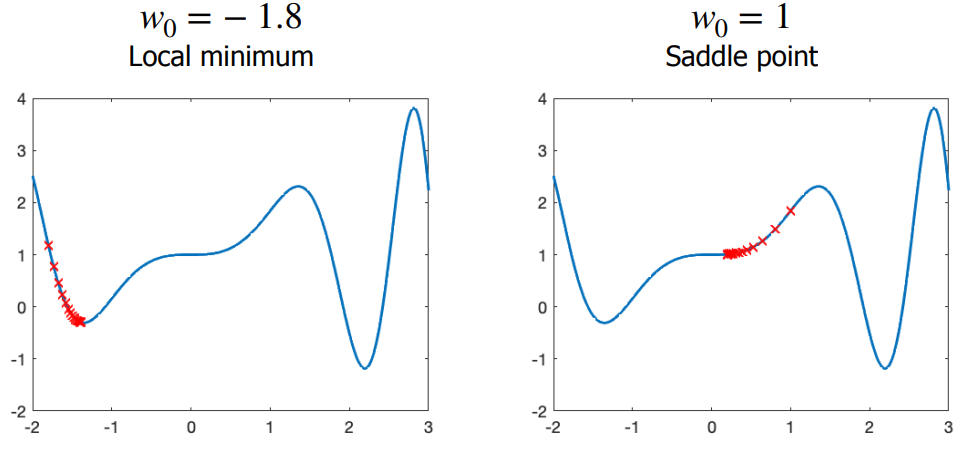
\includegraphics[width=0.5\linewidth]{images/img_20260304_200302.png}
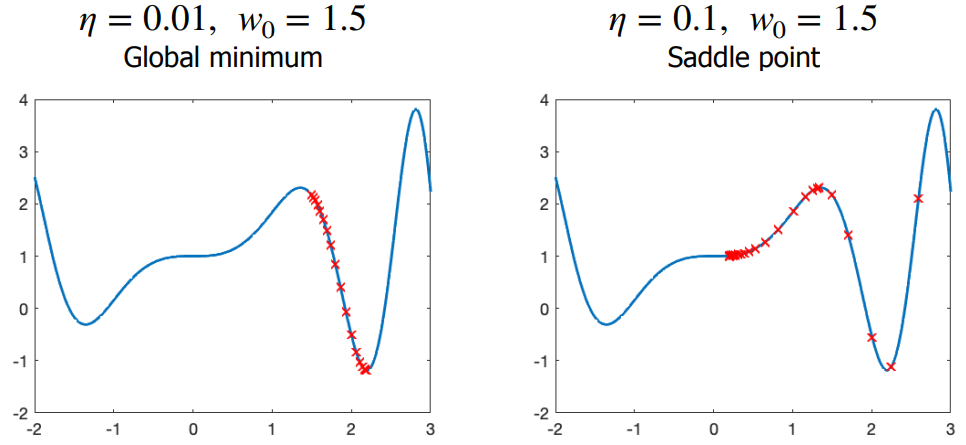
\includegraphics[width=0.5\linewidth]{images/img_20260304_200321.png}
\textbf{D dimensions case}
As in practice we have more than one parameter (i.e \textbf{w} $\in \mathbb{R}^{D+1}$), we use the function gradient: \[
  \nabla_w R(w) = \begin{pmatrix}
  \frac{\partial R}{\partial w^{(0)}} \\
   \frac{\partial R}{\partial w^{(1)}} \\
   \vdots \\
   \frac{\partial R}{\partial w^{(D)}} 
  \end{pmatrix}
  \in \mathbb{R}^D
\]
Recap : the gradient at a point w has the direction of the greatest increase of the function at w and its magnitude is the rate of increase in that direction. \\
So to decrease the function we therefore move in the direction opposite to the gradient. 
\\
\textbf{Gradient descent} is used to find the $argmin$ of a function, i.e., we want to find the values of parameters $x$ such that a function $f$ is minimized : \[
  x^* = \operatorname*{argmin}_xf(x)
\]
\textbf{Algorithm - gradient descent}
\begin{itemize}
  \item 1. Initialize $w_0$ (e.g, randomly)
  \item 2. While not converged \implies  update $ w_k \leftarrow w_{k-1} - \eta \nabla_w R(w_{k-1})$
\end{itemize}

\textbf{Cross-Entropy (multiple outputs)}: \[
  R(w) = - \sum_{i = 1}^N y_iln \sigma(w^Tx_i) + (1 - y_i)ln(1 - \sigma(w^Tx_i)) 
\]
\[
  = - \sum_{i \in positive samples} ln \sigma(w^Tx_i) - \sum_{i \in negative samples} ln(1 - \sigma(w^Tx_i))
\]
To minimize it via gradient descent we compute its gradient w.r.t \textbf{w} \[
  \nabla_w R(w) = \sum_{i=1}^{N} (\hat{y_i} - y_i) x_i 
\]
where $y_i$ is the true label for sample $i$, i.e., 1 for positive samples and 0 for negative samples. 
\begin{wrapfigure}{r}{0.3\linewidth}
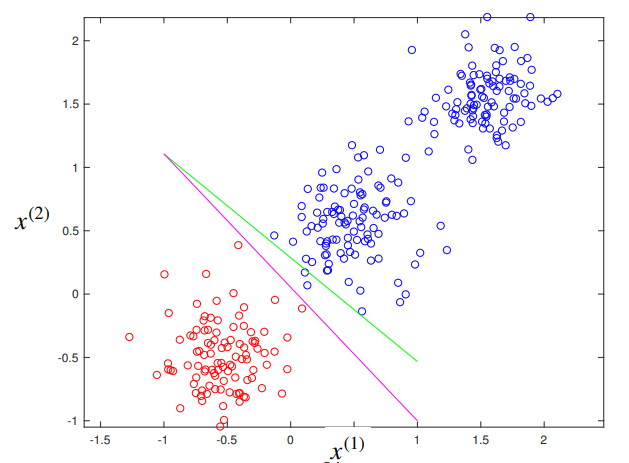
\includegraphics[width=\linewidth]{images/img_20260304_202817.png}
\end{wrapfigure}

And now, even with outliers, the boundary remains correct (Least-square classification in green, logistic regresion in magenta)

\subsection{Difference between linear models}
The real difference between linear models is the \textbf{loss function}, it has an impact on the resulting algorithm.

\subsection{Support Vector Machine (SVM)}
The SVM is a binary classifier based on the linear model as before: \[
  \hat{y} = w^Tx
\]

\begin{wrapfigure}{r}{0.3\linewidth}
  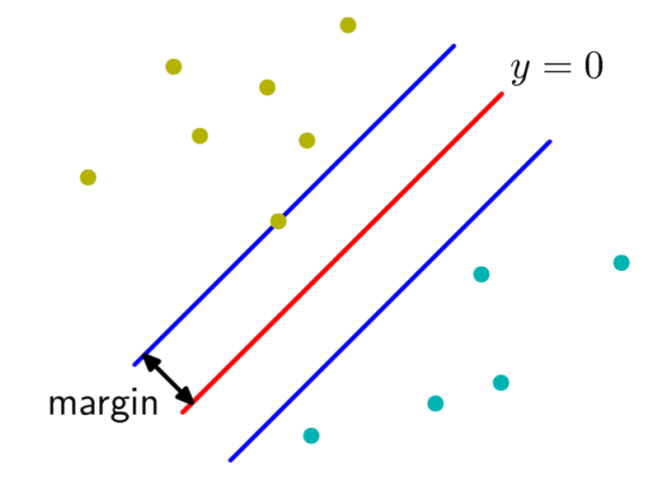
\includegraphics[width=\linewidth]{images/img_20260304_203955.png}
\end{wrapfigure}


It aims to maximize the margin (the distance between the decision boundary and the nearest sample) as a good decision boundary should maximize it, while enforcing a correct classification for each training samples. \\

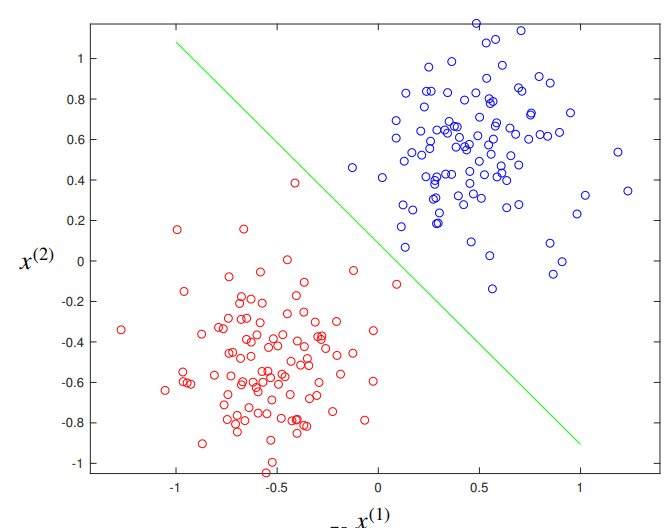
\includegraphics[width=0.4\linewidth]{images/img_20260304_203720.png}
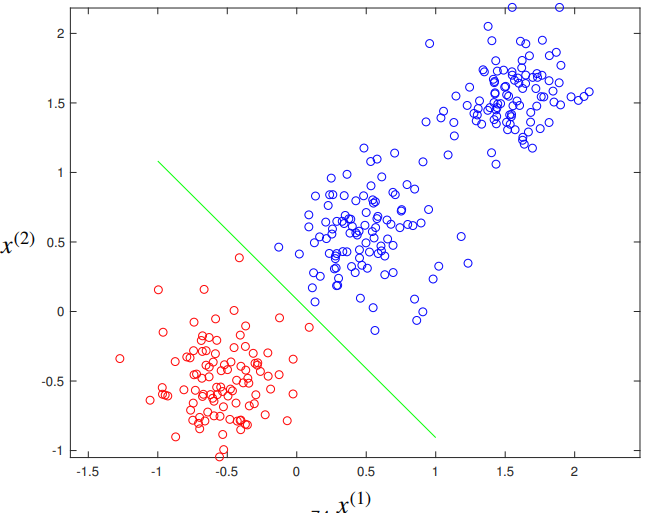
\includegraphics[width=0.4\linewidth]{images/img_20260304_203757.png}

So here we see that adding a new samples does not change the decision boundary as the margin stay the same.
